

\documentclass[tikz,border=3.14mm]{standalone}
\usetikzlibrary{positioning,chains}
\begin{document}


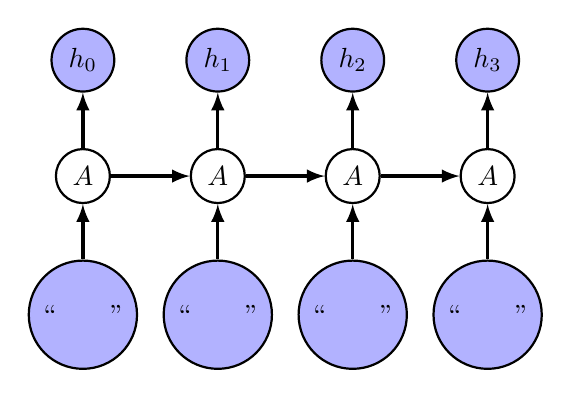
\begin{tikzpicture}[item/.style={circle,draw,thick,align=center},
itemc/.style={item,on chain,join}]
 \begin{scope}[start chain=going right,nodes=itemc,every
 join/.style={-latex,very thick},local bounding box=chain]
 \path node (A0) {$A$} node (A1) {$A$} node (A2) {$A$} node (A3)
 {$A$};
 \end{scope}

 \foreach \X in {0,1,2,3} 
 {\draw[very thick,-latex] (A\X.north) -- ++ (0,2em)
 node[above,item,fill=blue!30] (h\X) {$h_\X$};
 \draw[very thick,latex-] (A\X.south) -- ++ (0,-2em)
 node[below,item,fill=blue!30] (x\X) {``$\qquad$"};}

\end{tikzpicture}


\end{document}
